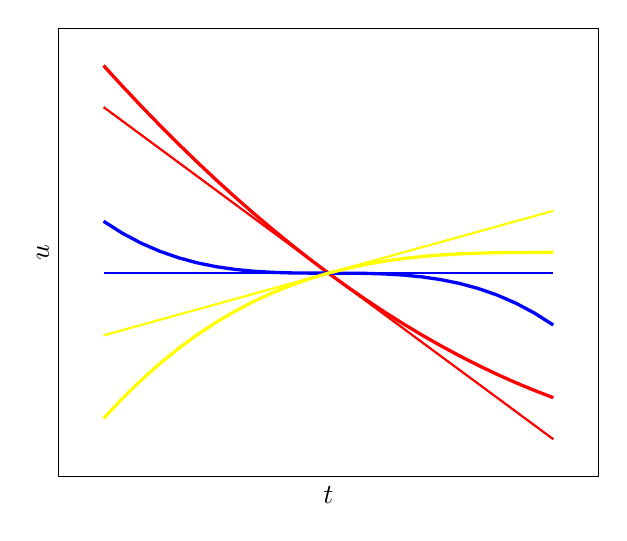
\begin{tikzpicture}
  \begin{axis}[ticks=none,xlabel=$t$,ylabel=$u$]
    \addplot[Red,very thick,domain=-0.5:0.5] {2.*(x-1.)^2 -2. +5.};
    \addplot[Red,thick,domain=-0.5:0.5] {-4.*x+5.};
    \addplot[Blue,very thick,domain=-0.5:0.5] {-5.*x^3+5.};
    \addplot[Blue,thick,domain=-0.5:0.5] {5.};
    \addplot[Yellow,very thick,domain=-0.5:0.5] {2.*(x-0.5)^3+(2.*(0.5)^3)+5.};
    \addplot[Yellow,thick,domain=-0.5:0.5] {1.5*x+5.};
    % \addplot3[black,very thick,domain=-5:5,samples=60,samples y=0]({x},{0.},{x^2+5.});
  \end{axis}
\end{tikzpicture}
%%% Local Variables:
%%% mode: latex
%%% TeX-master: "../../mainManuscript"
%%% End:
